% Vietnamese translation for OI Public Library
% Source-PDF: IOI中国国家候选队论文/2003/伍昱/由对称性解2-SAT问题.pdf
\documentclass[11pt]{article}
\usepackage{tikz}
\usetikzlibrary{arrows.meta,positioning}
\usepackage{oipl-vn}
\renewcommand{\figurename}{Hình}

\title{Giải bài toán 2-SAT bằng tính đối xứng}
\author{Ngũ Dục}
\date{}

\begin{document}
\maketitle
\sourcepath{IOI national candidate team papers / 2003 / Wu Yu / Symmetric 2-SAT}

\begin{abstract}
Nguồn là một bộ slide dạng ảnh về cách khai thác tính đối xứng trong bài toán
2-SAT. Bản tiếng Việt này chuyển nội dung slide thành một bài ghi chú có cấu
trúc, giữ ví dụ Peaceful Commission, đồ thị kéo theo, lập luận đối xứng và
thuật toán xây dựng nghiệm.
\end{abstract}

\section{Mở đầu}

2-SAT là một lớp đặc biệt của bài toán quyết định logic. Câu hỏi tự
nhiên là: lớp bài toán này có tính chất riêng nào, và có thể khai thác
các tính chất đó để giải hiệu quả ra sao? Tài liệu này bắt đầu từ một
bài toán ví dụ, sau đó rút ra một phương pháp tổng quát dựa trên tính
đối xứng của đồ thị kéo theo.

\section{Ví dụ: Peaceful Commission}

Bài toán \textit{Peaceful Commission} của POI 0106 được phát biểu như
sau. Một quốc gia có $n$ đảng, mỗi đảng có đúng hai đại biểu. Cần lập
một ủy ban hòa bình thỏa mãn hai điều kiện:
\begin{itemize}
  \item từ mỗi đảng chọn đúng một đại biểu;
  \item nếu hai đại biểu không thân thiện với nhau thì không được cùng
  xuất hiện trong ủy ban.
\end{itemize}

Các đại biểu được đánh số từ $1$ đến $2n$. Hai đại biểu $2a-1$ và $2a$
thuộc đảng thứ $a$. Dữ liệu gồm số đảng $n$, số cặp không thân thiện
$m$, rồi $m$ cặp chỉ số đại biểu khác nhau. Ràng buộc là
$1 \le n \le 8000$ và $0 \le m \le 20000$. Cần xác định có thể lập ủy
ban hay không; nếu có thì in ra một cách chọn.

Ví dụ, với ba đảng và hai cặp không thân thiện:
\begin{verbatim}
3 2
1 3
2 4
\end{verbatim}
một kết quả hợp lệ là:
\begin{verbatim}
1
4
5
\end{verbatim}

\section{Mô hình nhóm hai lựa chọn}

Ta có thể phát biểu lại bài toán dưới dạng sau. Có $n$ nhóm, nhóm thứ
$i$ gồm hai điểm $A_i$ và $A_i'$. Từ mỗi nhóm phải chọn đúng một điểm.
Một số cặp điểm là không tương thích, nghĩa là không thể chọn đồng thời.
Mục tiêu là chọn $n$ điểm sao cho mọi cặp điểm được chọn đều tương thích.

Ký hiệu $A_i'$ luôn là lựa chọn còn lại trong cùng nhóm với $A_i$. Khi
nói đến một điểm $A_i$, điểm đối ứng trong nhóm đó được viết là $A_i'$.

\section{Đồ thị kéo theo}

Nếu $A_i$ và $A_j$ không tương thích, thì việc chọn $A_i$ bắt buộc ta
phải chọn $A_j'$; tương tự, chọn $A_j$ bắt buộc ta phải chọn $A_i'$.
Do đó ta thêm hai cung:
\[
  A_i \to A_j', \qquad A_j \to A_i'.
\]
Hai cung này có tính đối xứng. Nói cách khác, nếu tồn tại cung
$A_i \to A_j$, thì nhất định tồn tại cung đối xứng
$A_j' \to A_i'$.

Trong ví dụ có bốn nhóm, giả sử các cặp không tương thích là
$(1,4)$, $(2,3)$ và $(7,3)$. Nếu ban đầu chọn $1$, các cung kéo theo
có thể buộc chọn $3$, từ đó không thể chọn $2$; tiếp theo buộc chọn
$8$, nên $4$ và $7$ cũng không được chọn. Các lựa chọn $5$ và $6$ khi
đó vẫn còn tự do.

\begin{figure}[ht]
\centering
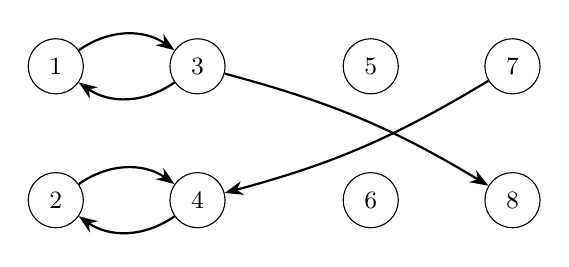
\begin{tikzpicture}[
  >=Stealth,
  v/.style={circle,draw,minimum size=7mm,inner sep=1pt,font=\small},
  every node/.style={font=\small},
  arc/.style={->,thick}
]
\node[v] (n1) at (0,1.1) {$1$};
\node[v] (n3) at (1.8,1.1) {$3$};
\node[v] (n2) at (0,-.6) {$2$};
\node[v] (n4) at (1.8,-.6) {$4$};
\node[v] (n5) at (4,1.1) {$5$};
\node[v] (n7) at (5.8,1.1) {$7$};
\node[v] (n6) at (4,-.6) {$6$};
\node[v] (n8) at (5.8,-.6) {$8$};
\draw[arc,bend left=35] (n1) to (n3);
\draw[arc,bend left=35] (n3) to (n1);
\draw[arc,bend left=35] (n2) to (n4);
\draw[arc,bend left=35] (n4) to (n2);
\draw[arc] (n3) to[bend left=8] (n8);
\draw[arc] (n7) to[bend left=8] (n4);
\end{tikzpicture}
\caption{Đồ thị kéo theo của ví dụ bốn nhóm: chọn \(1\) kéo theo \(3\), rồi kéo theo \(8\); do đó \(2,4,7\) bị loại, còn \(5,6\) chưa bị quyết định.}
\end{figure}

Một mâu thuẫn xuất hiện khi có một lựa chọn $A_i$ vừa bị buộc chọn vừa
bị cấm chọn. Thuật toán trực tiếp có thể thử lần lượt từng cặp chưa xác
định: chọn một trong hai điểm, lan truyền các hệ quả; nếu không mâu
thuẫn thì giữ lựa chọn đó, nếu có mâu thuẫn thì thử điểm còn lại. Nếu
cả hai đều mâu thuẫn thì bài toán vô nghiệm. Cách này đúng nhưng trong
trường hợp xấu nhất mất $O(nm)$, chưa khai thác đầy đủ tính đối xứng
của các cung.

\section{Co các thành phần liên thông mạnh}

Trong đồ thị kéo theo, nếu nhiều điểm nằm trên cùng một chu trình có
hướng, thì chọn một điểm trong chu trình sẽ buộc chọn tất cả các điểm
trong chu trình. Vì vậy ta co mỗi thành phần liên thông mạnh thành một
đỉnh mới. Sau khi co, ta thu được một đồ thị có hướng không chu trình
(DAG). Đồ thị mới tương đương với đồ thị ban đầu đối với việc suy luận
các kéo theo.

Với mỗi cung $A_i \to A_j$ của đồ thị ban đầu, giả sử $A_i$ thuộc
thành phần $S_i$ và $A_j$ thuộc thành phần $S_j$. Nếu $S_i \ne S_j$,
ta thêm cung
\[
  S_i \to S_j
\]
trong đồ thị co.

\begin{figure}[ht]
\centering
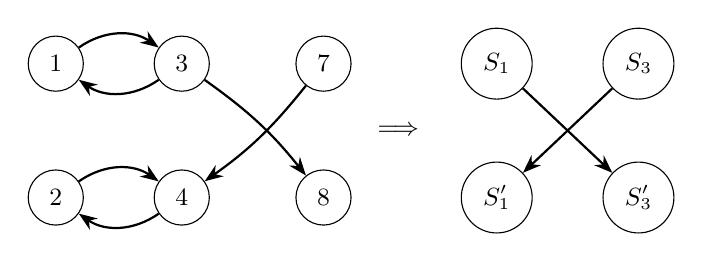
\begin{tikzpicture}[
  >=Stealth,
  v/.style={circle,draw,minimum size=7mm,inner sep=1pt,font=\small},
  c/.style={circle,draw,minimum size=9mm,inner sep=1pt,font=\small},
  every node/.style={font=\small},
  arc/.style={->,thick}
]
\node[v] (n1) at (0,1.1) {$1$};
\node[v] (n3) at (1.6,1.1) {$3$};
\node[v] (n2) at (0,-.6) {$2$};
\node[v] (n4) at (1.6,-.6) {$4$};
\node[v] (n7) at (3.4,1.1) {$7$};
\node[v] (n8) at (3.4,-.6) {$8$};
\draw[arc,bend left=35] (n1) to (n3);
\draw[arc,bend left=35] (n3) to (n1);
\draw[arc,bend left=35] (n2) to (n4);
\draw[arc,bend left=35] (n4) to (n2);
\draw[arc] (n3) to[bend left=8] (n8);
\draw[arc] (n7) to[bend left=8] (n4);
\node at (4.35,.25) {$\Longrightarrow$};
\node[c] (s1) at (5.6,1.1) {$S_1$};
\node[c] (s1p) at (5.6,-.6) {$S_1'$};
\node[c] (s3) at (7.4,1.1) {$S_3$};
\node[c] (s3p) at (7.4,-.6) {$S_3'$};
\draw[arc] (s1) -- (s3p);
\draw[arc] (s3) -- (s1p);
\end{tikzpicture}
\caption{Co hai chu trình \(\{1,3\}\) và \(\{2,4\}\) thành hai thành phần đối ứng \(S_1,S_1'\); các cung giữa thành phần tạo thành một DAG.}
\end{figure}

Sau phép co, bài toán có tiêu chuẩn vô nghiệm rất rõ ràng: nếu tồn tại
một cặp lựa chọn đối ứng $A_i$ và $A_i'$ thuộc cùng một thành phần liên
thông mạnh, thì không thể có nghiệm. Ngược lại, nếu không có cặp nào
như vậy thì bài toán có nghiệm.

\section{Tính đối xứng của đồ thị co}

Đồ thị ban đầu có tính chất truyền đối xứng: từ $A_i \to A_k$ suy ra
$A_k' \to A_i'$. Tính chất này vẫn đúng sau khi co thành phần liên
thông mạnh. Nếu hai đỉnh $S_i$ và $S_i'$ là hai thành phần đối ứng, thì
các hậu duệ của $S_i$ đối xứng với các tiền bối của $S_i'$.

Cụ thể, với mọi cặp $S_i, S_i'$, tập các đỉnh đi được từ $S_i$ tương
ứng với tập các đỉnh có đường đi đến $S_i'$. Do đó, nếu chọn $S_i$ thì
mọi hậu duệ của $S_i$ đều phải được chọn, còn $S_i'$ và mọi tiền bối
của $S_i'$ đều phải bị loại. Nhờ tính đối xứng này, thao tác loại bỏ
không tạo ra mâu thuẫn nếu tiêu chuẩn ở trên đã được thỏa mãn.

\begin{figure}[ht]
\centering
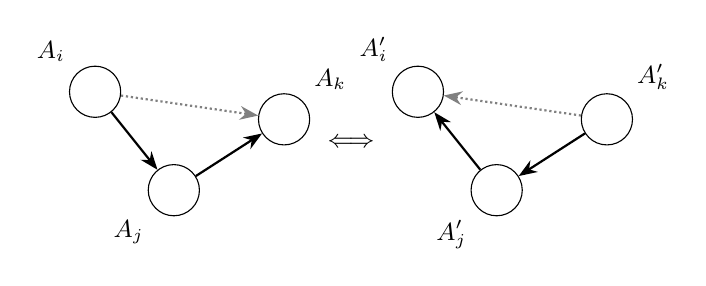
\begin{tikzpicture}[
  >=Stealth,
  p/.style={circle,draw,minimum size=6.5mm,inner sep=1pt,font=\small},
  every node/.style={font=\small},
  arc/.style={->,thick}
]
\node[p] (ai) at (0,1) {};
\node[p] (aj) at (1,-.25) {};
\node[p] (ak) at (2.4,.65) {};
\node[above left=1pt of ai] {$A_i$};
\node[below left=1pt of aj] {$A_j$};
\node[above right=1pt of ak] {$A_k$};
\draw[arc] (ai) -- (aj);
\draw[arc] (aj) -- (ak);
\draw[arc,densely dotted,gray] (ai) -- (ak);
\node at (3.25,.35) {$\Longleftrightarrow$};
\node[p] (aip) at (4.1,1) {};
\node[p] (ajp) at (5.1,-.25) {};
\node[p] (akp) at (6.5,.65) {};
\node[above left=1pt of aip] {$A_i'$};
\node[below left=1pt of ajp] {$A_j'$};
\node[above right=1pt of akp] {$A_k'$};
\draw[arc] (akp) -- (ajp);
\draw[arc] (ajp) -- (aip);
\draw[arc,densely dotted,gray] (akp) -- (aip);
\end{tikzpicture}
\caption{Đối xứng truyền: nếu \(A_i\to^* A_k\) qua một chuỗi kéo theo, thì chuỗi đối ứng \(A_k'\to^* A_i'\) cũng tồn tại.}
\end{figure}

\section{Xây dựng nghiệm}

Ta xét một bước tương tự thuật toán trực tiếp. Nếu chọn $S_i$, thì mọi
đỉnh $S_j$ với đường đi $S_i \to S_j$ đều phải được chọn. Đồng thời
$S_i'$ không được chọn, và mọi tiền bối của $S_i'$ cũng không được
chọn. Theo tính đối xứng của đồ thị co, việc xóa các đỉnh không được
chọn này không làm mất khả năng xây dựng nghiệm.

Mỗi lần ta tìm một cặp chưa xác định $S_i, S_i'$, chọn phía sao cho
không tồn tại đường đi $S_i \to S_i'$, rồi chọn $S_i$ và các hậu duệ
của nó, đồng thời loại $S_i'$ và các tiền bối của $S_i'$. Lặp lại quá
trình này cho đến khi mọi cặp đã được quyết định, ta thu được một
nghiệm.

\begin{figure}[ht]
\centering
\begin{tikzpicture}[
  >=Stealth,
  s/.style={circle,draw,minimum size=8mm,inner sep=1pt,font=\small},
  every node/.style={font=\small},
  arc/.style={->,thick}
]
\node[s] (s1) at (0,1.2) {$S_1$};
\node[s] (s2) at (2,1.2) {$S_2$};
\node[s] (s3) at (4,1.2) {$S_3$};
\node[s] (s1p) at (0,-1.1) {$S_1'$};
\node[s] (s2p) at (2,-1.1) {$S_2'$};
\node[s] (s3p) at (4,-1.1) {$S_3'$};
\draw[arc,red!70!black,bend left=25] (s1) to (s2);
\draw[arc,red!70!black,bend left=25] (s2p) to (s1p);
\draw[arc,blue!65!black,bend right=18] (s1) to (s3);
\draw[arc,blue!65!black,bend left=20] (s3) to (s3p);
\draw[arc,blue!65!black,bend right=18] (s3p) to (s1p);
\node[anchor=west] at (5.1,.65) {ví dụ chọn \(S_3'\)};
\node[anchor=west] at (5.1,.15) {chọn thêm hậu duệ \(S_1'\)};
\node[anchor=west] at (5.1,-.35) {loại \(S_3\) và tiền bối \(S_1\)};
\end{tikzpicture}
\caption{Các cung đỏ và xanh là hai chuỗi đối xứng. Chọn một thành phần sẽ chọn các hậu duệ của nó và loại thành phần đối ứng cùng các tiền bối.}
\end{figure}

Nếu mỗi lần phải tìm một đỉnh chưa xác định một cách mù quáng thì chi
phí có thể cao. Thay vào đó, ta sắp xếp topo đồ thị co và xử lý theo
thứ tự từ đáy lên. Khi đó có thể bỏ qua bước ``chọn toàn bộ hậu duệ'',
vì các hậu duệ đã được xử lý trước đó trong thứ tự này.

Ví dụ, một thứ tự topo từ đáy lên có thể là
\[
  S_1',\ S_2,\ S_2',\ S_3',\ S_3,\ S_1 .
\]
Xử lý theo thứ tự này, khi gặp một thành phần chưa được quyết định, ta
chọn nó và loại thành phần đối ứng của nó.

\section{Thuật toán}

Thuật toán cuối cùng gồm các bước sau:
\begin{enumerate}
  \item Dựng đồ thị kéo theo từ các cặp không tương thích.
  \item Tìm các thành phần liên thông mạnh của đồ thị.
  \item Co mỗi thành phần thành một đỉnh, rồi dựng đồ thị DAG tương
  ứng.
  \item Nếu có $A_i$ và $A_i'$ nằm trong cùng một thành phần, kết luận
  vô nghiệm và dừng.
  \item Sắp xếp topo đồ thị DAG.
  \item Duyệt các thành phần theo thứ tự topo từ đáy lên; nếu một
  thành phần chưa được quyết định, chọn nó và loại thành phần đối ứng.
  \item Từ các thành phần được chọn, xuất ra đại biểu tương ứng của
  từng nhóm.
\end{enumerate}

Các bước dựng đồ thị, tìm thành phần liên thông mạnh, co đồ thị và sắp
xếp topo đều tuyến tính theo kích thước đồ thị. Do đó độ phức tạp thời
gian của toàn bộ thuật toán xấp xỉ $O(m)$, hiệu quả hơn nhiều so với
cách thử trực tiếp.

\section{Kết luận}

Điểm then chốt của phương pháp là khai thác từ ``đối xứng''. Khi phát
hiện và sử dụng đúng tính chất đặc biệt của đồ thị kéo theo, ta có thể
giải bài toán 2-SAT một cách gọn và hiệu quả. Các bài toán được chuyển
về mô hình 2-SAT cũng có thể xử lý bằng cùng phương pháp.

Rộng hơn, việc đào sâu tính chất của đồ thị thường đem lại lời giải
mạnh hơn. Tư tưởng này không chỉ hữu ích trong lý thuyết đồ thị mà còn
có thể áp dụng cho nhiều bài toán khác: nắm chắc thuật toán cơ bản,
phân tích linh hoạt và mạnh dạn khai thác cấu trúc riêng của bài toán.

\end{document}
